\chapter{Data}\label{chap:data}
\begin{chapabstract}

In this chapter, I describe the dataset used for our study.
In Section~\ref{sec:HerschelReferenceSurvey}, I introduce the Herschel Reference Survey Catalog \citep{Boselli2010}.
Here, I explain how they choose galaxies for the catalog and previous studies for them.
In Section~\ref{sec:gleamsurvey}, I introduce the GaLactic Extragalactic All-sky MWA survey which we obtained the radio data for galaxy samples.

\end{chapabstract}

\section{Herschel Reference Survey (HRS)}\label{sec:HerschelReferenceSurvey}
In this section, I introduce the Herschel Reference Survey (HRS) catalog \citep{Boselli2010} which we selected galaxy samples from.
This survey is one of the Herschel guaranteed time key projects and originally it was compiled for understanding dust properties and interstellar medium in nearby galaxies.
The catalog is a publicly available and contains 322 galaxies selected with three criteria as follows:

\begin{enumerate}
    \item Volume-limitated:\\
        They choose galaxies whose distance from the earth is between $15$ and $25\,\mr{Mpc}$.
        This limitation reduce the distance uncertainty due to the galaxy peculiar motions and the selection effect due to the high-z galaxies.
        The lower limit ($15\,\mr{Mpc}$) also helps us to observe sources within the reasonable exposure time because galaxies too close to us are extended and we need too much time for the observation.
    \item $K$-band selection:\\
        They choose galaxies whose 2MASS $K$-band total magnitudes are brighter than $12\,\mr{mag}$ for star-forming and peculiar galaxies (Sa-Sd-Im-BCD), and $8.7\,\mr{mag}$ for quiescent galaxies (E, S0, S0a).
        If there are galaxies whose $K$-band magnitude darker than those values, their measurements are not regarded as an accurate photometry because of not enough exposure time.
        The reason why they have selected quiescent galaxies with the more stringent $K$-band selection criteria is these galaxies are expected to have low dust contents, and it is difficult to detect within the reasonable exposure time.
    \item High galactic latitude:\\
        They choose galaxies whose galactic latitude is high enough to minimize the contamination from the galactic center ($b > +55^{\circ}$).
        Also, they select galaxies with the low galactic extinction ($A\msb{B} < 0.2$; \citealt{Schlegel1998}).
\end{enumerate}

The selected galaxies locate in the sky region between $10\msu{h}17\msu{m}< \mr{R.A.}(2000) < 14\msu{h}43\msu{m}$ and $-6^{\circ} < \mr{decl.} < 60^{\circ}$ (Figure~\ref{fig:Boselli2010_figure1}).
HRS galaxies spans a wide range of the galaxy density environment from the center of Virgo cluster to the isolated region.
As a definition, we can regard the HRS sample as a ideal one for studying the galaxy environment.

\begin{figure}[htbp]
	\centering
	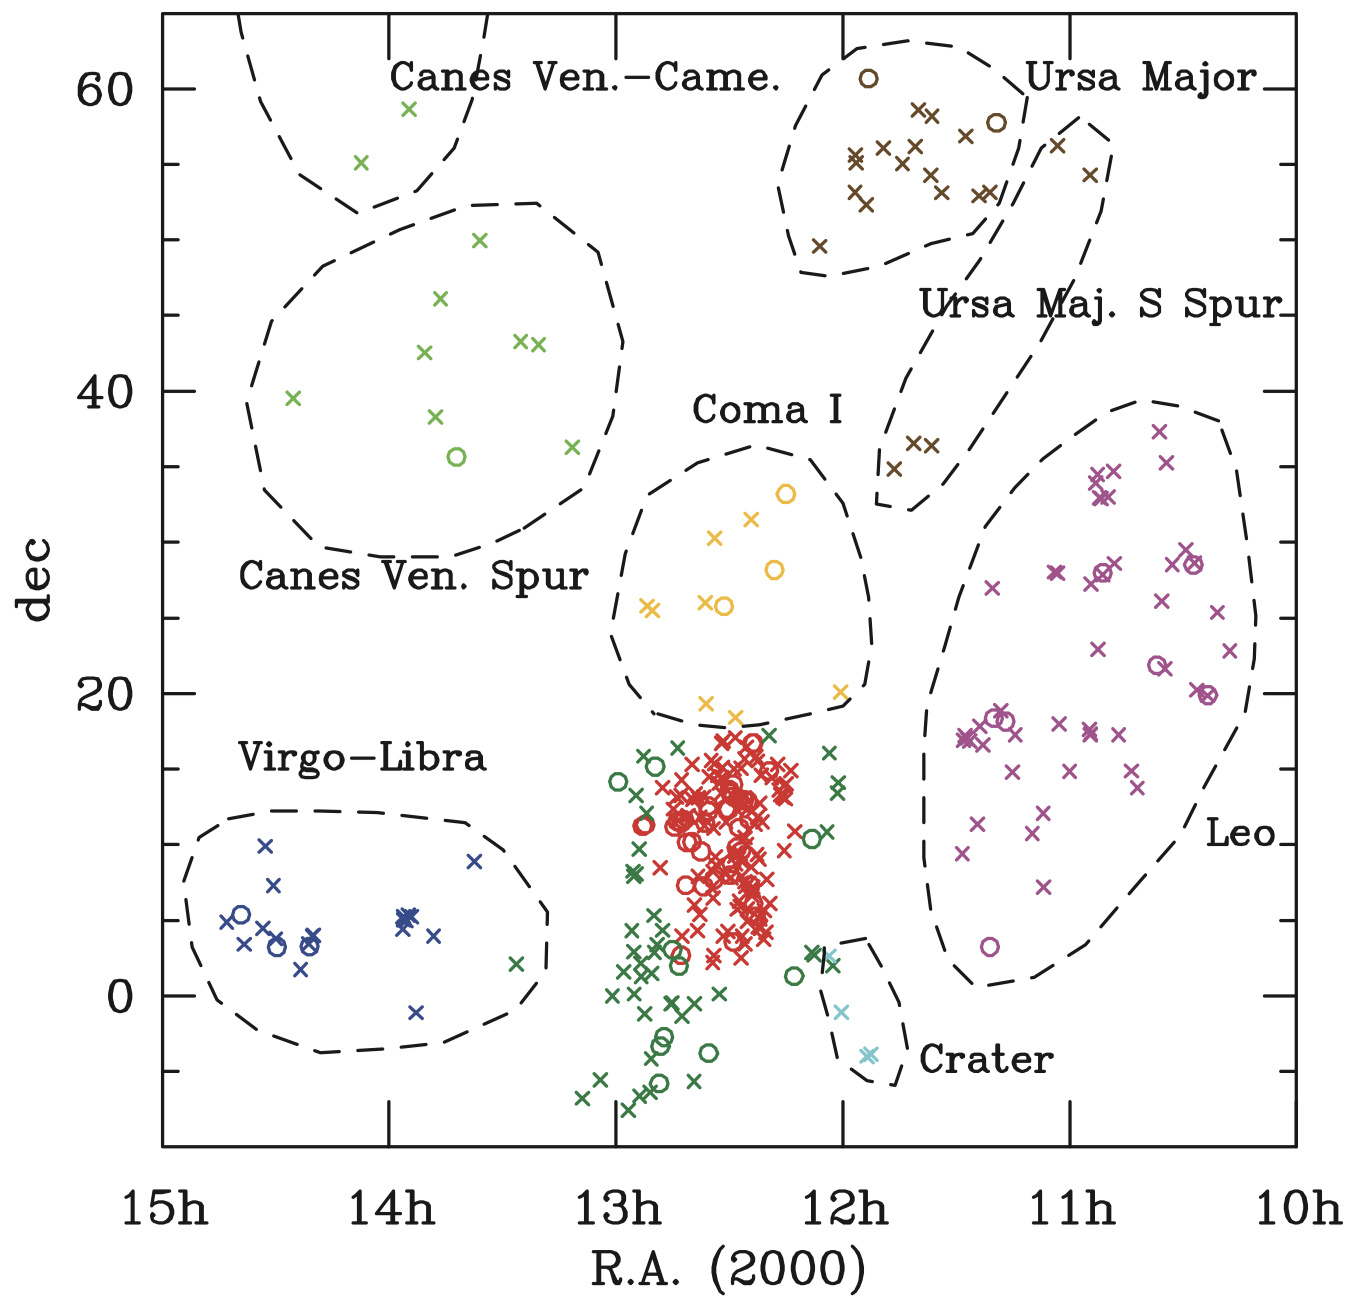
\includegraphics[width=.7\linewidth]{Chapter_3/Figures/Boselli2010_Figure1.png}
    \caption[Reprint from Boselli et al. 2010 (Figure~1)]{\label{fig:Boselli2010_figure1}
        (Reprint from Boselli et al. 2010, Figure~1)\\
        This figure shows the sky distribution of HRS galaxy samples.
        They show the early-type galaxies (E, S0, S0a) and late-type galaxies with circles and crosses, respectively.
        Dashed circles represents the different cloud regions. Each name of the cloud is shown close to each region.
        The red and dark green markers are Virgo galaxies (red: Virgo center, dark green: its outskirts).
    }
\end{figure}

In addition to a wide range of the environment, HRS galaxies distribute a wide range of the galaxy morphology (Figure~\ref{fig:Boselli2010_figure2}).

\begin{figure}[htbp]
	\centering
	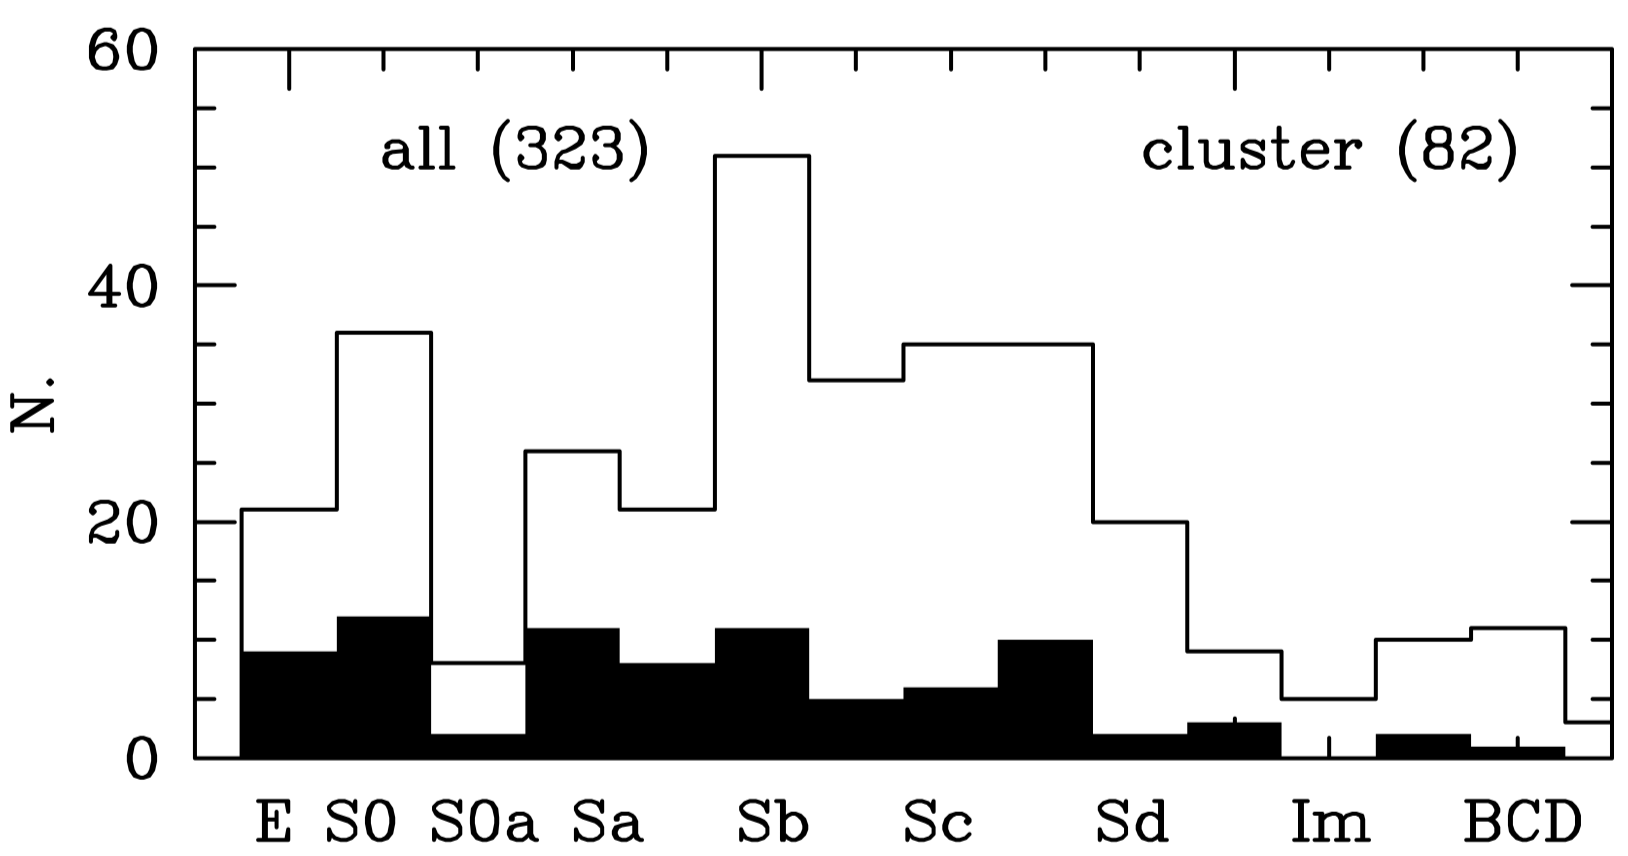
\includegraphics[width=.8\linewidth]{Chapter_3/Figures/Boselli2010_Figure2.png}
    \caption[Reprint from Boselli et al. 2010 (Figure~2)]{\label{fig:Boselli2010_figure2}
        (Reprint from Boselli et al. 2010, Figure~2)\\
        This figure shows the distribution in the morphology-type of HRS galaxies.
        The shaded histogram represents the distribution in it of only the cluster sample.
        Here, the cluster sample composed of HRS galaxies located in the Virgo A and B clouds.
    }
\end{figure}

Since HRS galaxies are supposed to be well-represented for the whole galaxy population located in the local universe, investigating their physical properties is crucial to understand them.
After \citet{Boselli2010} published the HRS catalog, many studies investigating the physical properties for HRS galaxies have been done until now.
Here, I introduce some of the studies for the HRS sample.
\citet{Cortese2012} investigated their UV and optical properties using the Galaxy Evolution Explorer ({\it GALEX\/};~\citealt{Martin2005}) and SDSS-DR7 \citep{Abazajian2009}.
\citet{Boselli2014} studied their cold gas properties with $^{12}\mr{CO}\brp{1-0}$ observed by the Kitt Peak 12m radio telescope and obtained from the literature data.
They also investigate the \nh~gas obtained from The Arecibo Legacy Fast ALFA (ALFALFA;~\citealt{Giovanelli2005, Haynes2011}) survey.
\citet{Ciesla2014} executed the SED fitting for HRS galaxies with Code Investigating GALaxy Emission (CIGALE;~\citealt{Noll2009}).

Thanks to all of previous research about the HRS sample, they are well-studied among a wide range of the wavelength from the X-ray to the radio emission at $1.5\GHz$.
However, the low-frequency around $100\MHz$ is not examined so far.
Since we extend the wavelength range of the HRS sample to around $100\MHz$, in this study, we focus on a subsample of HRS galaxies whose counterpart is detected by the latest low-frequency survey (Section~\ref{sec:gleamsurvey}).



\section{GLEAM survey}\label{sec:gleamsurvey}

In this section, I introduce the GaLactic Extragalactic All-sky MWA (GLEAM) survey \citep{Hurley-Walker2017a} which we obtained the radio continuum data from.
This survey was operated by the Murchison Widefield Array (MWA) telescope in Western Australia \citep{Tingay2013a}.
It observed a whole southern sky and a northern sky up to $+30^{\circ}$ ($\sim$25,000 $\mathrm{\deg}^2$;~Figure~\ref{fig:HurleyWalker2017_figure11}).
The catalog from this survey is a publicly-available and contains 307,455 detected radio sources with fluxes at 20 narrow bands between $72$ and $231\MHz$ (each band has $7.68\MHz$ band width).
The sensitivity and angular resolution at $200\MHz$ are $\sim 7\,\mr{mJy}$ and $\sim 2\,\mr{arcmin}$ respectively.
The completeness of this survey at $200\MHz$ is $90\%$ at $\sim 170\mr{mJy}$.
Since this survey allows us to examine the low-frequency spectral energy distribution accurately with its 20 narrow bands, we adopt the radio source catalog for our study.

\begin{figure}[htbp]
	\centering
	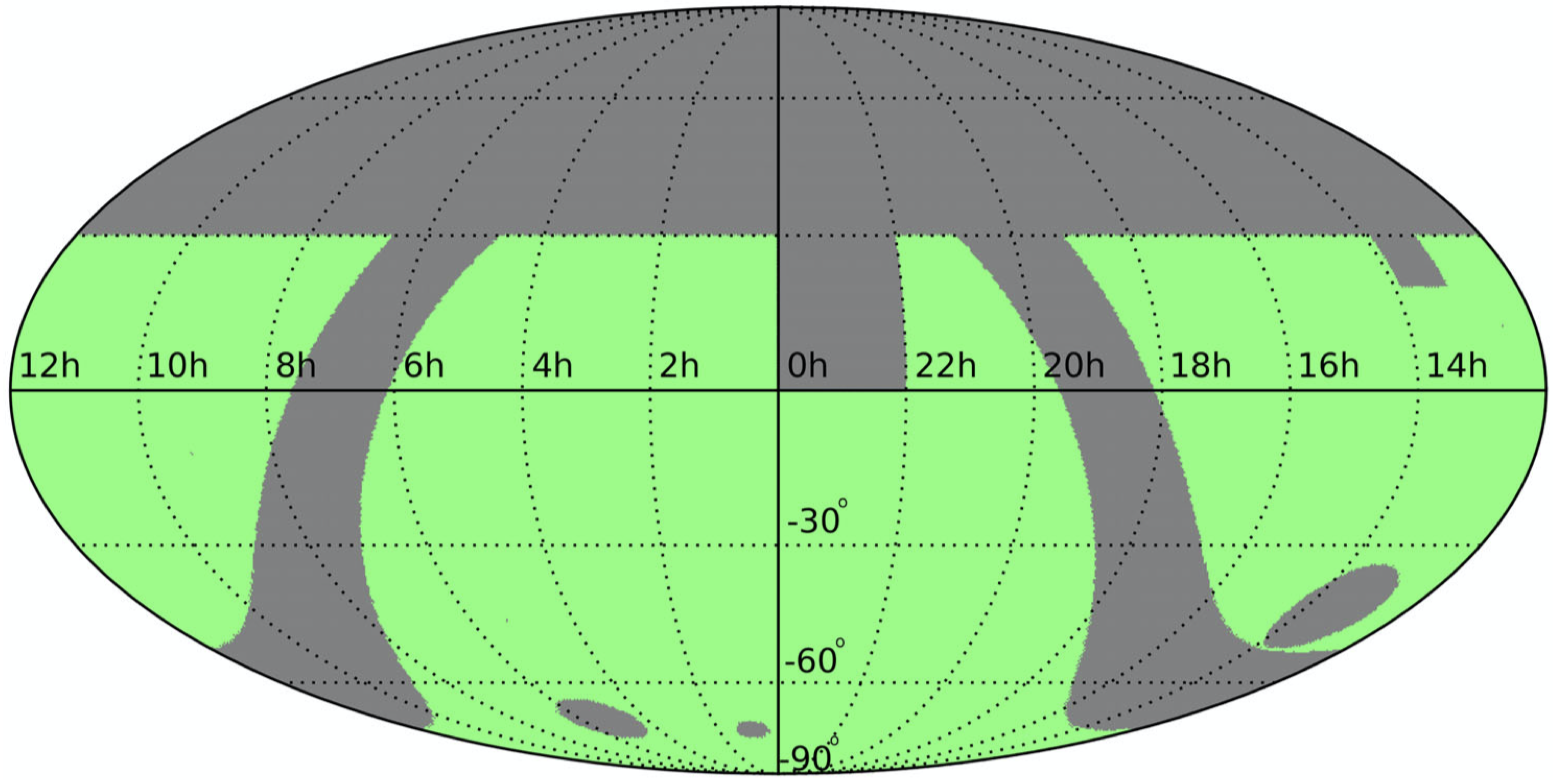
\includegraphics[width=.7\linewidth]{Chapter_3/Figures/HurleyWalker_Figure11.png}
    \caption[Reprint from Hurley-Walker et al. 2017 (Figure~11)]{\label{fig:HurleyWalker2017_figure11}
        (Reprint from Hurley-Walker et al. 2017, Figure~11)\\
        This figure shows the observed area by the GLEAM survey (green shaded region).
        \citet{Hurley-Walker2017a} exclude several regions intentionally to minimize the contamination:
        Galactic plane (Absolute Galactic latitude $<10^{\circ}$),
        Ionospherically distorted ($0^{\circ} < \mr{Dec} < +30^{\circ}\ \mr{and}\ 22\msu{h} < \mr{R.A.} < 0\msu{h}$),
        Centaurus A ($13\msu{h}25\msu{m}28\msu{s}\ -43^{\circ}01'09'',\,r=9^{\circ}$),
        Sidelobe reflection of Cen A ($20^{\circ} < \mr{Dec} < +30^{\circ}\ \mr{and}\ 13\msu{h}07\msu{m} < \mr{R.A.} < 13\msu{h}53\msu{m}$),
        Large Magellanic Cloud ($05\msu{h}23\msu{m}35\msu{s}\ -69^{\circ}45'22'',\,r=5.5^{\circ}$) and Small Magellanic Cloud ($00\msu{h}52\msu{m}38\msu{s}\ -72^{\circ}48'01'',\,r=2.5^{\circ}$).
    }
\end{figure}






%\bibliographystyle{mnras}
%%\bibliography{example} % if your bibtex file is called example.bib
%\bibliography{masterthesis}
